\documentclass[11pt]{beamer}
\usepackage{cmap}
\usepackage[utf8]{inputenc}
\usepackage[T1]{fontenc}
\usetheme{Singapore}
\usepackage{graphicx}
\usepackage{multicol}
\usepackage{booktabs}
\usepackage{amsfonts,amsbsy}
\usepackage{float}
\usepackage{tikz}
\usetikzlibrary{arrows.meta,positioning}
\usepackage{hyperref}

% Colores y comandos
\newcommand{\hlr}[1]{\textcolor{red}{#1}}
\newcommand{\hlb}[1]{\textcolor{blue}{#1}}
\newcommand{\hlg}[1]{\textcolor{green!50!black}{#1}}

\title[FinHive]{FinHive: \\ De la Teoria a la Practica en Arquitecturas Multiagente}
\subtitle{Un sistema jerarquico de analisis financiero, construido sobre Databricks}
\author{Matias Fabian Adell}
\institute{Portfolio project --- \url{github.com/matiasadell/finhive}}
\date{\today}

\begin{document}

\begin{frame}[plain]
    \maketitle
\end{frame}

%%%%%%%%%%%%%%%%%%%%%%%
\section{Motivacion}

\begin{frame}{De una investigacion teorica a un sistema real}
\begin{itemize}
    \item Punto de partida: un timeline propio de \textbf{24 arquitecturas agenticas}
    (2020--2026), organizado en seis eras narrativas --- de RAG clasico a los primeros
    intentos de sistematizar el campo.
    \item La pregunta que atraviesa esas seis eras: \hlb{cuanto control de diseno se le
    devuelve al propio sistema} --- topologia, memoria, tolerancia a fallos.
    \item FinHive es el ejercicio deliberado de aplicar esa cadena completa a un dominio
    real, en vez de quedarse en el nivel conceptual.
    \item Un modelo individual no alcanza para un dominio tan heterogeneo como las
    finanzas: macro, equities, riesgo de portfolio, noticias, cripto --- cada uno con
    sus propias fuentes y formatos.
\end{itemize}
\end{frame}

%%%%%%%%%%%%%%%%%%%%%%%
\section{Arquitectura}

\begin{frame}{Supervisor de supervisores: jerarquia de dos niveles}
\centering
\resizebox{0.98\linewidth}{!}{%
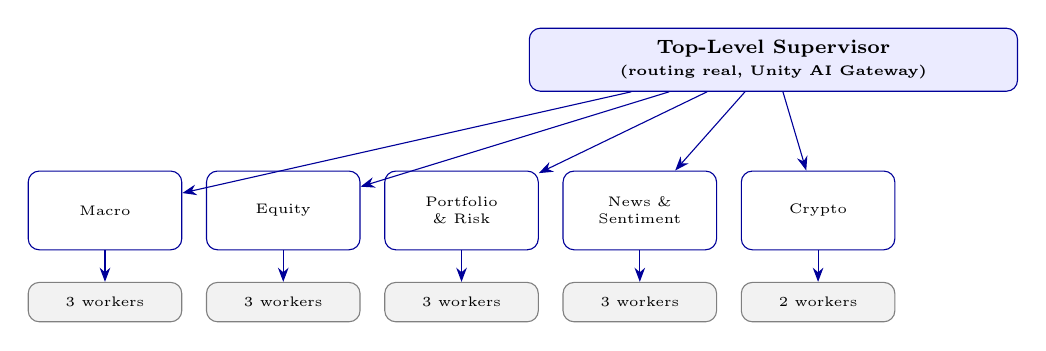
\begin{tikzpicture}[
  node distance=7mm and 3mm,
  every node/.style={font=\tiny},
  sup/.style={draw=blue!60!black, fill=blue!8, rounded corners, minimum width=6.2cm,
              minimum height=8mm, align=center, font=\scriptsize\bfseries},
  dom/.style={draw=blue!60!black, fill=white, rounded corners, minimum width=1.95cm,
              minimum height=10mm, align=center, font=\tiny},
  wrk/.style={draw=gray, fill=gray!10, rounded corners, minimum width=1.95cm,
              minimum height=5mm, align=center, font=\tiny},
  arr/.style={-{Stealth[length=1.8mm]}, draw=blue!60!black}
]
\node[sup] (top) {Top-Level Supervisor \\ \tiny (routing real, Unity AI Gateway)};

\node[dom, below left=10mm and 44mm of top] (macro) {Macro};
\node[dom, right=3mm of macro] (equity) {Equity};
\node[dom, right=3mm of equity] (pf) {Portfolio\\\& Risk};
\node[dom, right=3mm of pf] (news) {News \&\\Sentiment};
\node[dom, right=3mm of news] (crypto) {Crypto};

\draw[arr] (top) -- (macro);
\draw[arr] (top) -- (equity);
\draw[arr] (top) -- (pf);
\draw[arr] (top) -- (news);
\draw[arr] (top) -- (crypto);

\node[wrk, below=4mm of macro] (m1) {3 workers};
\node[wrk, below=4mm of equity] (e1) {3 workers};
\node[wrk, below=4mm of pf] (p1) {3 workers};
\node[wrk, below=4mm of news] (n1) {3 workers};
\node[wrk, below=4mm of crypto] (c1) {2 workers};

\draw[arr] (macro) -- (m1);
\draw[arr] (equity) -- (e1);
\draw[arr] (pf) -- (p1);
\draw[arr] (news) -- (n1);
\draw[arr] (crypto) -- (c1);
\end{tikzpicture}%
}

\vspace{4mm}
\begin{itemize}
    \item Mismo patron replicado en dos niveles: un supervisor decide, con
    \emph{structured output}, a que nodo delegar --- hasta \texttt{FINISH}.
    \item \hlg{13 workers ReAct} sobre \hlg{25 tools} registradas en Unity Catalog.
\end{itemize}
\end{frame}

\begin{frame}{Cinco dominios especializados}
\footnotesize
\begin{tabular}{@{}p{0.24\linewidth}p{0.70\linewidth}@{}}
\toprule
\textbf{Dominio} & \textbf{Fuente de datos / especialidad} \\
\midrule
Macro & FRED (tasas, inflacion, indicadores) \\
Equity Research & yfinance + SEC EDGAR (fundamentals, filings XBRL) \\
Portfolio \& Risk & \textbf{Computo propio}: VaR, volatilidad, Sharpe, correlacion (numpy/pandas) \\
News \& Sentiment & Alpha Vantage (sentiment estructurado) + Tavily (fallback CRAG) \\
Crypto \& Alt & CoinGecko (precio, tendencias, ranking) \\
\bottomrule
\end{tabular}
\end{frame}

\begin{frame}{Stack: 100\% sobre Databricks Free Edition}
\begin{itemize}
    \item \textbf{Foundation Model APIs nativos}: Llama 3.3 70B / 3.1 8B --- \hlg{sin
    ninguna key externa}.
    \item \textbf{Unity Catalog Functions}: 25 tools gobernadas, alternativa sin costo a
    los Managed MCP servers.
    \item \textbf{Unity AI Gateway}: routing real entre modelos + rate limits.
    \item \textbf{Databricks Repos}: repo de GitHub conectado, notebook demo corriendo
    dentro del workspace.
    \item \textbf{MLflow Tracing}: cada invocacion, cada tool call, trazado.
\end{itemize}

\vspace{3mm}
\begin{center}
\textcolor{blue}{\Large Costo total verificado: \textbf{\$0}}
\end{center}
\end{frame}

%%%%%%%%%%%%%%%%%%%%%%%
\section{Teoria aplicada}

\begin{frame}{De paper a decision de ingenieria}
\scriptsize
\begin{tabular}{@{}p{0.30\linewidth}p{0.64\linewidth}@{}}
\toprule
\textbf{Concepto} & \textbf{Donde vive en FinHive} \\
\midrule
ReAct (Yao et al., 2022) & Los 13 workers hoja \\
Corrective RAG & Fallback a Tavily cuando Alpha Vantage no alcanza \\
Multi-Agent Supervisor / Jerarquica (TalkHier) & Los dos niveles de la topologia completa \\
Mixture-of-Agents & Sintesis cuando una pregunta cruza 2+ dominios \\
MCP (concepto) & Unity Catalog Functions gobernadas, sin el costo del servicio gestionado \\
LLM Gateway & Unity AI Gateway: routing, rate limits, usage tracking \\
\bottomrule
\end{tabular}
\end{frame}

%%%%%%%%%%%%%%%%%%%%%%%
\section{Lo que realmente fallo}

\begin{frame}{Hallazgo: un bug de plataforma causa una alucinacion}
\textbf{El problema:} el modo recomendado para tools de Unity Catalog
(\texttt{UCFunctionToolkit local}) genera un subproceso que hace
\texttt{import resource} --- \hlr{modulo que solo existe en Unix}. En Windows falla
silenciosamente.

\vspace{3mm}
\textbf{La consecuencia real:} el worker, sin dato, \hlr{alucino una cifra plausible}
(5.25\% de tasa de fondos federales) en vez de admitir el fallo. El valor real,
verificado por separado: \hlg{3.63\%}.

\vspace{4mm}
\begin{center}
\textcolor{blue}{\large ``Un fallo silencioso de tool es indistinguible de un dato real.''}
\end{center}
\end{frame}

\begin{frame}{Hallazgo: ruteo entre dominios y su costo real}
\begin{itemize}
    \item Pregunta: \emph{``¿cuando es el proximo earnings de Apple?''}
    \item Se enruto a \textbf{Equity} en vez de \textbf{News \& Sentiment} --- el router
    solo veia \emph{nombres} de equipo, sin limites explicitos.
    \item Equity, sin la tool de calendario, \hlr{alucino una fecha incorrecta} (2025 en
    vez de 2026).
\end{itemize}

\vspace{3mm}
\textbf{Correccion:} descripciones explicitas por equipo, con lineas de
``\emph{esto NO es de este equipo}'' en los casos de frontera --- aplicado
preventivamente al sumar el quinto dominio, antes de que apareciera el mismo bug.
\end{frame}

%%%%%%%%%%%%%%%%%%%%%%%
\section{Model Routing}

\begin{frame}{Unity AI Gateway: routing real, verificado empiricamente}
\texttt{finhive\_router}: 70\% del trafico a Llama 3.3 70B, 30\% a GPT OSS 120B.

\vspace{3mm}
\textbf{No solo configurado --- verificado con 6 llamadas reales:}

\vspace{2mm}
\begin{center}
\begin{tabular}{cccccc}
\toprule
1 & 2 & 3 & 4 & 5 & 6 \\
\midrule
Llama & Llama & Llama & \hlr{GPT-OSS} & Llama & Llama \\
\bottomrule
\end{tabular}
\end{center}

\vspace{3mm}
\texttt{ChatDatabricks} todavia no soporta este path nuevo de API --- se resolvio con el
cliente OpenAI-compatible (\texttt{langchain\_openai.ChatOpenAI}) que Databricks expone
directamente, sin esperar a la libreria especializada.
\end{frame}

%%%%%%%%%%%%%%%%%%%%%%%
\section{Resultados}

\begin{frame}{Resultados}
\begin{itemize}
    \item \hlg{5 dominios} completos, verificados extremo a extremo contra APIs reales.
    \item \hlg{13 workers ReAct} sobre \hlg{25 Unity Catalog Functions}.
    \item \hlg{6 tests de integracion} --- cada uno verifica \emph{grounding} real, no
    solo ausencia de excepciones.
    \item \hlg{\$0} de costo total de LLM y embeddings, verificado en vivo.
    \item \hlg{10 ADRs} documentando cada decision y cada hallazgo con su razonamiento.
\end{itemize}
\end{frame}

\begin{frame}{Trabajo futuro}
\begin{itemize}
    \item Guardrails formales (topico, seguridad, \emph{groundedness}) --- motivados
    directamente por los hallazgos de este proyecto.
    \item Memoria persistente (patron MemGPT).
    \item RAG estilo RAPTOR sobre el texto completo de 10-K/10-Q.
    \item Mosaic AI Agent Framework + evaluacion CLEARS.
    \item Demo desplegada como Databricks App.
\end{itemize}
\end{frame}

\begin{frame}[plain]
\centering
\textcolor{blue}{\Huge{¡Gracias!}}\\
\vspace{1em}
\textcolor{black}{\large Codigo completo, ADRs, y notebook demo:}\\
\vspace{0.5em}
\textcolor{blue}{\Large \url{github.com/matiasadell/finhive}}\\
\vspace{1em}
\textcolor{black}{\normalsize ¿Preguntas o feedback? Bienvenidos.}
\end{frame}

\end{document}
